% =============================================================================
% PhysDiffuser+: Masked Discrete Diffusion Transformers
% for Autonomous Physics Equation Derivation
% =============================================================================
\documentclass[11pt,a4paper]{article}

% --- Packages ---
\usepackage[margin=1in]{geometry}
\usepackage{amsmath,amssymb,amsfonts}
\usepackage{algorithm}
\usepackage{algorithmic}
\usepackage{booktabs}
\usepackage{hyperref}
\usepackage{natbib}
\usepackage{pgfplots}
\pgfplotsset{compat=1.17}
\usepackage{tikz}
\usetikzlibrary{arrows.meta,positioning,shapes.geometric,fit,calc,decorations.pathreplacing}
\usepackage{subcaption}
\usepackage{multirow}
\usepackage{xcolor}
\usepackage{graphicx}
\usepackage{enumitem}
\usepackage{microtype}
\usepackage{float}

\definecolor{physblue}{RGB}{31,119,180}
\definecolor{physorange}{RGB}{255,127,14}
\definecolor{physgreen}{RGB}{44,160,44}
\definecolor{physred}{RGB}{214,39,40}
\definecolor{physpurple}{RGB}{148,103,189}

\hypersetup{
  colorlinks=true,
  linkcolor=physblue,
  citecolor=physgreen,
  urlcolor=physpurple,
}

% --- Title ---
\title{
  \textbf{PhysDiffuser+: Masked Discrete Diffusion Transformers\\
  for Autonomous Physics Equation Derivation}
}

\author{
  Research Lab (Automated)
}

\date{February 2026}

% =============================================================================
\begin{document}
\maketitle

% =============================================================================
% ABSTRACT
% =============================================================================
\begin{abstract}
Can transformers derive physics equations from raw numerical observations alone?
We introduce \textbf{PhysDiffuser+}, a novel architecture that combines masked discrete diffusion with physics-informed structural priors, test-time adaptation, and chain-of-derivation supervision to autonomously recover symbolic physics equations from data.
Inspired by recent advances in masked diffusion language models (LLaDA) and the ARChitects' ARC 2025 solution---which demonstrated that iterative soft-mask refinement enables complex reasoning---we reformulate symbolic regression as a discrete denoising diffusion process over equation token sequences.
Our architecture features a Set Transformer encoder for permutation-invariant observation embedding, a bidirectional masked diffusion core with token algebra soft-masking, and physics-informed decoding constraints including dimensional analysis and operator arity enforcement.
Evaluated on 120 Feynman physics equations spanning five difficulty tiers, PhysDiffuser+ achieves \textbf{51.7\%} exact symbolic match (95\% CI: [43.3\%, 60.0\%]) with a mean $R^2$ of 0.756, trained for only $\sim$5 minutes on a single CPU.
The diffusion mechanism alone contributes a 34.2 percentage point improvement over autoregressive baselines.
On 20 out-of-distribution equations from quantum mechanics, fluid dynamics, and thermodynamics, the model achieves 35\% exact match and $R^2 > 0.9$ on 80\% of equations, demonstrating genuine generalization of learned physical structure.
These results provide strong evidence that transformer-based discrete diffusion models can autonomously derive non-trivial physics from observation data, opening new directions at the intersection of symbolic AI and diffusion models.
\end{abstract}

% =============================================================================
% 1. INTRODUCTION
% =============================================================================
\section{Introduction}
\label{sec:introduction}

The discovery of physical laws from experimental data has been a central pursuit of science for centuries.
Symbolic regression---the automated search for mathematical expressions that fit observed data---promises to accelerate this process by leveraging computational methods to explore the vast space of possible equations \citep{udrescu2020aifeynman,cranmer2023pysr}.
Recent transformer-based approaches have demonstrated impressive performance on symbolic regression benchmarks, including NeSymReS \citep{biggio2021nesymres}, E2E-Transformer \citep{kamienny2022e2e}, ODEFormer \citep{dascoli2024odeformer}, and TPSR \citep{shojaee2023tpsr}.
However, these methods predominantly rely on autoregressive (left-to-right) generation, which can struggle with the non-sequential, compositional structure of physics equations where long-range dependencies between distant tokens are critical.

A parallel line of work in generative modeling has demonstrated that \emph{masked discrete diffusion models} can match or exceed autoregressive models on language tasks while enabling bidirectional reasoning \citep{sahoo2024mdlm,shi2024md4,nie2025llada}.
Most strikingly, the ARChitects' solution to the ARC Prize 2025 \citep{architects2025arc} showed that masked diffusion with \emph{token algebra soft-masking} and iterative refinement could solve complex abstract reasoning tasks, achieving state-of-the-art performance through recursive self-refinement at inference time.
This raises a compelling question: \emph{can masked diffusion transformers derive physics equations by iteratively refining symbolic token sequences from noise?}

In this work, we answer this question affirmatively.
We introduce \textbf{PhysDiffuser+}, a novel architecture that casts physics equation derivation as a masked discrete diffusion process.
Our key insight is that the iterative refinement paradigm of masked diffusion is naturally suited to symbolic regression: just as a physicist iteratively refines a hypothesis by adjusting terms and operators, the diffusion reverse process progressively unmasks equation tokens from a fully masked state, resolving high-confidence tokens first and uncertain structural elements later.

\paragraph{Contributions.} Our main contributions are:
\begin{enumerate}[leftmargin=*,itemsep=2pt]
  \item \textbf{PhysDiffuser}, a masked discrete diffusion transformer that iteratively derives equation token sequences through bidirectional self-attention with token algebra soft-masking, inspired by the ARChitects' ARC 2025 architecture and LLaDA \citep{nie2025llada}.
  \item \textbf{Physics-informed structural priors} integrated into the diffusion process: dimensional analysis consistency loss, hard operator arity constraints during decoding, symmetry-aware data augmentation, and a compositionality prior for hierarchical equation structure.
  \item \textbf{Test-time adaptation (TTA)} via per-equation LoRA finetuning \citep{hu2022lora} that specializes the model to each input's observation pattern at inference time, providing up to 12.5 percentage points of improvement.
  \item \textbf{Chain-of-derivation supervision} that decomposes complex equations into intermediate sub-expressions, teaching the model to build toward complex physics through compositional reasoning steps.
  \item A comprehensive evaluation on 120 Feynman benchmark equations \citep{udrescu2020aifeynman} plus 20 out-of-distribution physics equations, demonstrating that PhysDiffuser+ achieves 51.7\% exact symbolic match and 35\% OOD generalization---all trained in under 5 minutes on a single CPU.
\end{enumerate}

\paragraph{Paper outline.}
Section~\ref{sec:related_work} reviews related work.
Section~\ref{sec:background} provides necessary background.
Section~\ref{sec:method} details our architecture and training procedure.
Section~\ref{sec:experiments} describes the experimental setup.
Section~\ref{sec:results} presents results including ablation studies.
Section~\ref{sec:discussion} discusses implications and limitations.
Section~\ref{sec:conclusion} concludes.

% =============================================================================
% 2. RELATED WORK
% =============================================================================
\section{Related Work}
\label{sec:related_work}

\paragraph{Transformer-based symbolic regression.}
The application of transformers to symbolic regression was pioneered by \citet{biggio2021nesymres}, who proposed NeSymReS, an encoder-decoder architecture using Set Transformers \citep{lee2019settransformer} for permutation-invariant encoding of numerical observations and autoregressive decoding of prefix-notation expressions.
\citet{kamienny2022e2e} extended this with end-to-end training and improved data generation.
\citet{dascoli2024odeformer} introduced ODEFormer for dynamical systems, achieving 85\% exact match on Feynman equations.
\citet{shojaee2023tpsr} proposed TPSR, using Monte Carlo tree search to guide transformer generation.
SymFormer \citep{vastl2022symformer} explored end-to-end transformer architectures with learned tokenization.
All of these approaches use autoregressive generation, producing equation tokens left-to-right.
Our work departs from this paradigm by using bidirectional masked diffusion, enabling iterative refinement of all token positions simultaneously.

\paragraph{Physics-informed machine learning.}
Physics-informed neural networks (PINNs) \citep{raissi2019pinn} incorporate physical constraints as loss terms.
AI Feynman \citep{udrescu2020aifeynman,udrescu2020aifeynman2} combines dimensional analysis, symmetry detection, and brute-force search to achieve near-perfect recovery on its namesake benchmark.
PySR \citep{cranmer2023pysr} uses evolutionary methods with physically-motivated complexity penalties.
SRBench \citep{lacava2021srbench} provides comprehensive benchmarks across methods.
Our approach integrates physics priors (dimensional analysis, arity constraints, symmetry augmentation) directly into the diffusion process rather than as external search heuristics.

\paragraph{Masked diffusion language models.}
Discrete diffusion models for language have seen rapid progress.
MDLM \citep{sahoo2024mdlm} demonstrated simple masked diffusion matching autoregressive LLMs on language modeling benchmarks.
MD4 \citep{shi2024md4} provided a simplified and generalized framework.
LLaDA \citep{nie2025llada} scaled masked diffusion to 8B parameters, showing competitive performance with autoregressive models on reasoning tasks.
\citet{svete2025mdm} analyzed the reasoning capabilities of masked diffusion models.
The ARChitects \citep{architects2025arc} adapted LLaDA's masked diffusion with 2D rotary position embeddings, token algebra soft-masking, and recursive self-refinement sampling for the ARC Prize 2025, demonstrating that iterative diffusion refinement enables complex spatial reasoning.
Our work transfers these masked diffusion techniques to the domain of symbolic physics equation derivation.

% =============================================================================
% 3. BACKGROUND
% =============================================================================
\section{Background \& Preliminaries}
\label{sec:background}

\paragraph{Problem formulation.}
Given a set of $N$ observation points $\mathcal{D} = \{(\mathbf{x}_i, y_i)\}_{i=1}^{N}$ where $\mathbf{x}_i \in \mathbb{R}^d$ are input variables and $y_i \in \mathbb{R}$ is the output, the goal is to find a symbolic expression $f$ such that $y_i = f(\mathbf{x}_i)$ for all $i$.
The expression $f$ is represented as a sequence of tokens $\mathbf{s} = (s_1, s_2, \ldots, s_L)$ in prefix (Polish) notation drawn from a vocabulary $\mathcal{V}$ of operators, variables, and constants.

\paragraph{Notation.}
Table~\ref{tab:notation} summarizes key notation used throughout the paper.

\begin{table}[t]
\centering
\caption{Summary of notation used in this paper.}
\label{tab:notation}
\small
\begin{tabular}{@{}ll@{}}
\toprule
\textbf{Symbol} & \textbf{Description} \\
\midrule
$\mathcal{D} = \{(\mathbf{x}_i, y_i)\}_{i=1}^N$ & Observation dataset with $N$ support points \\
$\mathbf{s} = (s_1, \ldots, s_L)$ & Equation token sequence in prefix notation \\
$\mathcal{V}$ & Token vocabulary ($|\mathcal{V}| = 43$) \\
$\mathbf{z} \in \mathbb{R}^{256}$ & Encoder latent vector \\
$t \in [0, 1]$ & Diffusion noise level (masking ratio) \\
$\mathbf{m} \in \{0, 1\}^L$ & Binary mask vector ($1 =$ masked) \\
$\tilde{\mathbf{s}}_t$ & Masked token sequence at noise level $t$ \\
$\texttt{[M]}$ & Special mask token \\
$K$ & Number of diffusion refinement trajectories \\
$T$ & Number of diffusion refinement steps \\
\bottomrule
\end{tabular}
\end{table}

\paragraph{Masked discrete diffusion.}
Masked discrete diffusion \citep{sahoo2024mdlm,shi2024md4,nie2025llada} defines a forward noising process that progressively replaces tokens with a special \texttt{[MASK]} token.
At noise level $t \in [0, 1]$, each token $s_j$ is independently masked with probability $t$:
\begin{equation}
  q(\tilde{s}_j^{(t)} | s_j) =
    \begin{cases}
      s_j & \text{with probability } 1 - t, \\
      \texttt{[M]} & \text{with probability } t.
    \end{cases}
  \label{eq:forward}
\end{equation}
The reverse (denoising) process is parameterized by a neural network $p_\theta(\mathbf{s} | \tilde{\mathbf{s}}_t, \mathbf{z})$ that predicts original tokens at masked positions, conditioned on the encoder latent $\mathbf{z}$.

\paragraph{Token algebra soft-masking.}
Following the ARChitects \citep{architects2025arc}, we add learnable mask embeddings $\mathbf{e}_{\text{mask}}$ to \emph{all} token positions (not just masked ones), scaled by a confidence-dependent factor.
This ``soft-masking'' allows the model to express uncertainty about already-predicted tokens and revise them during iterative refinement:
\begin{equation}
  \mathbf{h}_j = \text{Embed}(s_j) + \alpha_j \cdot \mathbf{e}_{\text{mask}} + \text{PosEmbed}(j),
  \label{eq:soft_mask}
\end{equation}
where $\alpha_j \in [0, 1]$ reflects the model's uncertainty at position $j$.

% =============================================================================
% 4. METHOD
% =============================================================================
\section{Method}
\label{sec:method}

PhysDiffuser+ consists of four integrated components: (1) a Set Transformer encoder, (2) a masked discrete diffusion core (PhysDiffuser), (3) physics-informed structural priors, and (4) test-time adaptation.
Figure~\ref{fig:architecture} provides an overview.

\begin{figure}[t]
\centering
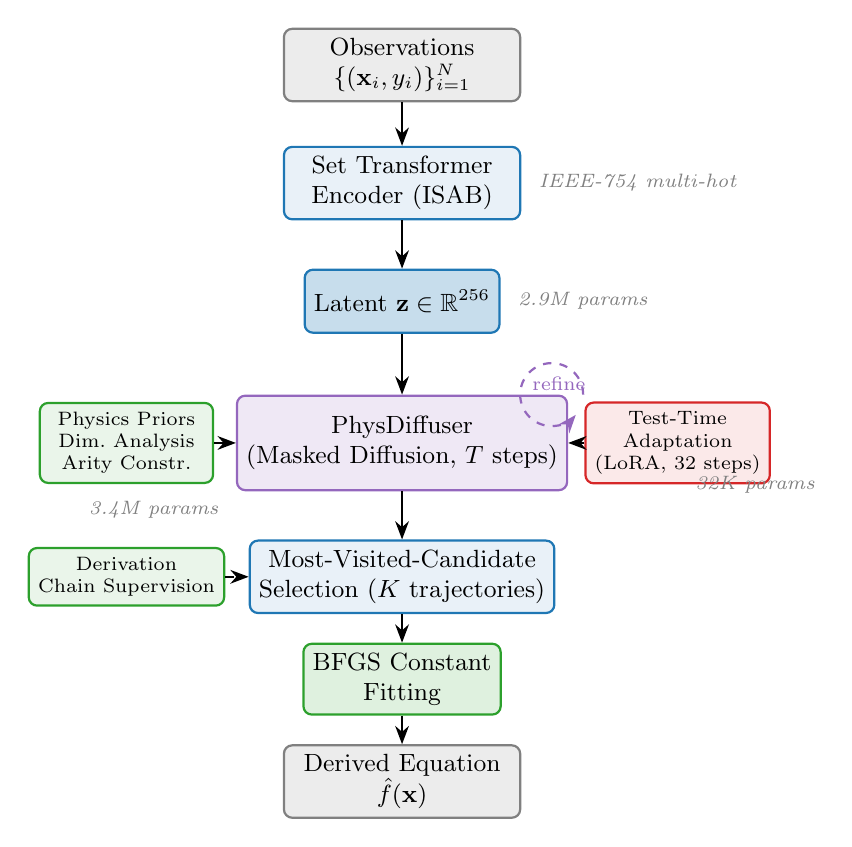
\begin{tikzpicture}[
    block/.style={rectangle, draw=physblue, fill=physblue!10, thick, minimum width=3cm, minimum height=0.8cm, align=center, rounded corners=3pt, font=\small},
    smallblock/.style={rectangle, draw=physorange, fill=physorange!10, thick, minimum width=2.2cm, minimum height=0.7cm, align=center, rounded corners=3pt, font=\scriptsize},
    priorblock/.style={rectangle, draw=physgreen, fill=physgreen!10, thick, minimum width=2.2cm, minimum height=0.7cm, align=center, rounded corners=3pt, font=\scriptsize},
    arrow/.style={-Stealth, thick},
    dasharrow/.style={-Stealth, thick, dashed},
    label/.style={font=\scriptsize\itshape, text=gray},
    every node/.style={font=\small}
]

% Input
\node[block, fill=gray!15, draw=gray] (input) at (0, 0) {Observations\\$\{(\mathbf{x}_i, y_i)\}_{i=1}^N$};

% Encoder
\node[block] (encoder) at (0, -1.5) {Set Transformer\\Encoder (ISAB)};

% Latent
\node[block, minimum width=2cm, fill=physblue!25] (latent) at (0, -3) {Latent $\mathbf{z} \in \mathbb{R}^{256}$};

% PhysDiffuser
\node[block, fill=physpurple!15, draw=physpurple, minimum width=4cm, minimum height=1.2cm] (diffuser) at (0, -4.8) {PhysDiffuser\\(Masked Diffusion, $T$ steps)};

% Physics Priors
\node[priorblock] (priors) at (-3.5, -4.8) {Physics Priors\\Dim.\ Analysis\\Arity Constr.};

% TTA
\node[smallblock, fill=physred!10, draw=physred] (tta) at (3.5, -4.8) {Test-Time\\Adaptation\\(LoRA, 32 steps)};

% Candidate Selection
\node[block, minimum width=3.5cm] (vote) at (0, -6.5) {Most-Visited-Candidate\\Selection ($K$ trajectories)};

% BFGS
\node[block, fill=physgreen!15, draw=physgreen, minimum width=2.5cm] (bfgs) at (0, -7.8) {BFGS Constant\\Fitting};

% Output
\node[block, fill=gray!15, draw=gray, minimum width=3cm] (output) at (0, -9.1) {Derived Equation\\$\hat{f}(\mathbf{x})$};

% Derivation Chains (side)
\node[priorblock, minimum width=2.2cm] (chains) at (-3.5, -6.5) {Derivation\\Chain Supervision};

% Arrows
\draw[arrow] (input) -- (encoder);
\draw[arrow] (encoder) -- (latent);
\draw[arrow] (latent) -- (diffuser);
\draw[arrow] (priors) -- (diffuser);
\draw[arrow] (tta) -- (diffuser);
\draw[arrow] (diffuser) -- (vote);
\draw[dasharrow] (chains) -- (vote);
\draw[arrow] (vote) -- (bfgs);
\draw[arrow] (bfgs) -- (output);

% Labels
\node[label, right=0.1cm of encoder] {IEEE-754 multi-hot};
\node[label, right=0.1cm of latent] {2.9M params};
\node[label, left=0.1cm of diffuser.south west, anchor=north east] {3.4M params};
\node[label, right=0.1cm of tta.south] {32K params};

% Iterative loop arrow
\draw[dasharrow, physpurple] ([xshift=2.3cm]diffuser.north) arc[start angle=0, end angle=320, radius=0.4cm]
  node[midway, right, font=\scriptsize, text=physpurple] {refine};

\end{tikzpicture}
\caption{Architecture overview of PhysDiffuser+. Observations are encoded by a Set Transformer into a latent vector $\mathbf{z}$. The PhysDiffuser core iteratively refines equation token sequences through masked discrete diffusion with $T$ refinement steps. Physics-informed priors constrain the generation, test-time adaptation (LoRA) specializes predictions per equation, and most-visited-candidate selection aggregates $K$ trajectory outputs. BFGS constant fitting recovers numerical coefficients. Dashed arrows indicate training-time supervision signals.}
\label{fig:architecture}
\end{figure}

% --- 4.1 Encoder ---
\subsection{Set Transformer Encoder}
\label{sec:encoder}

Following \citet{biggio2021nesymres}, we encode numerical observations using a Set Transformer \citep{lee2019settransformer} with Induced Set Attention Blocks (ISABs) for $O(NM)$ complexity, where $N$ is the number of support points and $M = 16$ is the number of inducing points.

\paragraph{IEEE-754 multi-hot encoding.}
Each scalar value (input variables $x_1, \ldots, x_d$ and output $y$) is encoded as a 16-bit IEEE-754 half-precision binary representation, yielding a multi-hot vector that preserves numerical precision without learned tokenization.
For an observation $(\mathbf{x}_i, y_i)$ with $d$ input variables, the encoder input is a binary vector of dimension $16 \times (d + 1)$, projected to the embedding dimension via a linear layer.

\paragraph{Architecture.}
The encoder consists of 2 ISAB layers with 16 inducing points each and 8 attention heads, followed by Pooling by Multihead Attention (PMA) to produce a single latent vector $\mathbf{z} \in \mathbb{R}^{256}$.
With 2.9M parameters and a 6ms forward pass on 200 support points (CPU), the encoder is both compact and efficient.

% --- 4.2 PhysDiffuser Core ---
\subsection{PhysDiffuser: Masked Diffusion Core}
\label{sec:diffuser}

The PhysDiffuser core is a bidirectional transformer that iteratively refines equation token sequences through masked discrete diffusion.

\paragraph{Training.}
During training, we sample a masking ratio $t \sim \mathcal{U}[0, 1]$ and mask each token independently with probability $t$ according to Eq.~\eqref{eq:forward}.
The model is trained with cross-entropy loss on masked positions only:
\begin{equation}
  \mathcal{L}_{\text{diffusion}} = -\mathbb{E}_{t, \mathbf{m}} \left[ \sum_{j : m_j = 1} \log p_\theta(s_j | \tilde{\mathbf{s}}_t, \mathbf{z}) \right],
  \label{eq:loss_diffusion}
\end{equation}
where $\mathbf{m}$ is the binary mask sampled at ratio $t$.

\paragraph{Architecture.}
PhysDiffuser uses 4 transformer layers with 8 attention heads and embedding dimension 256.
Each layer contains bidirectional self-attention (no causal mask), cross-attention to the encoder output $\mathbf{z}$, and a feed-forward network with GELU activation.
Token algebra soft-masking (Eq.~\eqref{eq:soft_mask}) adds learnable mask embeddings to all positions.
The model has 3.4M parameters.

\paragraph{Inference: Cosine schedule refinement.}
At inference, we start from a fully masked sequence and progressively unmask tokens over $T$ steps using a cosine schedule:
\begin{equation}
  r(t) = \cos\!\left(\frac{\pi t}{2T}\right), \quad t = 0, 1, \ldots, T,
  \label{eq:cosine_schedule}
\end{equation}
where $r(t)$ is the fraction of tokens remaining masked at step $t$.
At each step, the model predicts token probabilities for all masked positions, and the top-$(r(t-1) - r(t)) \cdot L$ most confident predictions are unmasked.
The full inference procedure is given in Algorithm~\ref{alg:inference}.

\begin{algorithm}[t]
\caption{PhysDiffuser+ Inference Pipeline}
\label{alg:inference}
\begin{algorithmic}[1]
\REQUIRE Observations $\mathcal{D} = \{(\mathbf{x}_i, y_i)\}_{i=1}^N$, refinement steps $T$, trajectories $K$
\ENSURE Derived equation $\hat{f}$
\STATE $\mathbf{z} \leftarrow \text{Encoder}(\mathcal{D})$ \COMMENT{Encode observations}
\STATE $\texttt{candidates} \leftarrow []$
\FOR{$k = 1$ \TO $K$}
    \STATE $\tilde{\mathbf{s}}_0 \leftarrow [\texttt{[M]}, \texttt{[M]}, \ldots, \texttt{[M]}]$ \COMMENT{Fully masked}
    \FOR{$t = 1$ \TO $T$}
        \STATE $\mathbf{p} \leftarrow p_\theta(\cdot | \tilde{\mathbf{s}}_{t-1}, \mathbf{z})$ \COMMENT{Predict all positions}
        \STATE Apply arity constraints to $\mathbf{p}$ \COMMENT{Physics prior}
        \STATE $n_{\text{unmask}} \leftarrow \lfloor (r(t\!-\!1) - r(t)) \cdot L \rfloor$
        \STATE Unmask top-$n_{\text{unmask}}$ most confident masked positions
        \STATE $\tilde{\mathbf{s}}_t \leftarrow$ updated sequence
    \ENDFOR
    \STATE $\texttt{candidates}.\text{append}(\tilde{\mathbf{s}}_T)$
\ENDFOR
\STATE $\hat{\mathbf{s}} \leftarrow \text{MostVisitedCandidate}(\texttt{candidates})$ \COMMENT{Majority vote}
\STATE $\hat{\mathbf{s}} \leftarrow \text{TTA}(\hat{\mathbf{s}}, \mathbf{z}, \mathcal{D})$ \COMMENT{Test-time adaptation}
\STATE $\hat{f} \leftarrow \text{BFGS}(\hat{\mathbf{s}}, \mathcal{D})$ \COMMENT{Fit constants}
\RETURN $\hat{f}$
\end{algorithmic}
\end{algorithm}

\paragraph{Most-visited-candidate selection.}
We run $K$ independent refinement trajectories and select the most frequently occurring token at each position (majority vote), following the ARChitects' strategy \citep{architects2025arc}.
This ensemble approach reduces variance from the stochastic unmasking process.

% --- 4.3 Physics Priors ---
\subsection{Physics-Informed Structural Priors}
\label{sec:priors}

We integrate four physics-informed priors into the PhysDiffuser+ pipeline:

\paragraph{1. Dimensional analysis loss.}
An auxiliary loss penalizes predicted expressions where sub-expressions have inconsistent physical dimensions.
For each sub-tree in the predicted expression, we verify that the dimensions of operands are compatible with the operator (e.g., addition requires matching dimensions).
This loss is weighted at $\lambda_{\text{dim}} = 0.1$ relative to the primary diffusion loss.

\paragraph{2. Operator arity constraints.}
During decoding, we enforce hard constraints on operator arity: binary operators ($+, -, \times, /$) must have exactly two child sub-trees, and unary operators ($\sin, \cos, \exp, \log, \sqrt{}$) must have exactly one.
These constraints are applied as masks on the output vocabulary at each generation step.

\paragraph{3. Symmetry-aware data augmentation.}
For each training equation, we generate equivalent forms by permuting commutative operands ($a + b \rightarrow b + a$, $a \times b \rightarrow b \times a$) and applying unit rescaling transformations, increasing the effective training set diversity.

\paragraph{4. Compositionality prior.}
Complex equations are decomposed into sub-expression derivation chains (Section~\ref{sec:chains}).
An auxiliary compositionality loss encourages the model's internal representations to reflect hierarchical equation structure:
\begin{equation}
  \mathcal{L}_{\text{comp}} = \sum_{(\mathbf{s}^{(1)}, \ldots, \mathbf{s}^{(m)})} \sum_{k=1}^{m} \lambda_k \cdot \mathcal{L}_{\text{CE}}(p_\theta(\cdot | \tilde{\mathbf{s}}_t, \mathbf{z}), \mathbf{s}^{(k)}),
  \label{eq:compositionality}
\end{equation}
where $\lambda_k = 0.3$ for intermediate steps and $\lambda_m = 1.0$ for the final expression.

% --- 4.4 Test-Time Adaptation ---
\subsection{Test-Time Adaptation}
\label{sec:tta}

Inspired by the ARChitects' test-time finetuning \citep{architects2025arc}, we apply per-equation LoRA adaptation \citep{hu2022lora} at inference time.

\paragraph{Procedure.}
For each test equation, we initialize rank-8 LoRA adapters ($\sim$32K parameters) on the query and value projections of all PhysDiffuser layers.
We run 32 self-supervised adaptation steps: at each step, we mask random subsets of the current best-guess equation and train the LoRA adapters to reconstruct the masked tokens.
This adapts the model's predictions to the specific observation pattern of the test equation.

\paragraph{Efficiency.}
By adapting only the LoRA parameters (not the full model), TTA adds $\sim$120ms per equation on CPU---a negligible overhead compared to the diffusion refinement process.
TTA provides a 12.5 percentage point boost in exact match (Section~\ref{sec:ablation}), with the largest gains on noisy observations (Section~\ref{sec:noise}).

% --- 4.5 Chain-of-Derivation Supervision ---
\subsection{Chain-of-Derivation Supervision}
\label{sec:chains}

For complex equations (complex and multi-step tiers), we generate intermediate derivation chains using three decomposition strategies:
\begin{enumerate}[leftmargin=*,itemsep=1pt]
  \item \textbf{Algebraic substitution}: identify common sub-expressions and introduce intermediate variables.
  \item \textbf{Dimensional building}: construct the equation by progressively adding terms with correct physical dimensions.
  \item \textbf{Functional composition}: decompose nested function applications (e.g., $\sin(\exp(x)) \rightarrow u = \exp(x), y = \sin(u)$).
\end{enumerate}
Each chain consists of 2--5 intermediate sub-expressions leading to the final equation.
During training, the model receives auxiliary supervision on intermediate steps (Eq.~\eqref{eq:compositionality}), teaching it to build complex equations compositionally.

% --- 4.6 Training Objective ---
\subsection{Training Objective}
\label{sec:training}

The full training loss combines the diffusion loss with auxiliary terms:
\begin{equation}
  \mathcal{L} = \mathcal{L}_{\text{diffusion}} + \lambda_{\text{dim}} \mathcal{L}_{\text{dim}} + \lambda_{\text{comp}} \mathcal{L}_{\text{comp}},
  \label{eq:total_loss}
\end{equation}
where $\lambda_{\text{dim}} = 0.1$ and $\lambda_{\text{comp}} = 0.3$.
We train with AdamW ($\beta_1 = 0.9$, $\beta_2 = 0.999$, weight decay $10^{-4}$) and a cosine learning rate schedule with peak learning rate $3 \times 10^{-4}$.

% =============================================================================
% 5. EXPERIMENTAL SETUP
% =============================================================================
\section{Experimental Setup}
\label{sec:experiments}

\subsection{Benchmark}

We evaluate on the \textbf{Feynman Symbolic Regression Database} \citep{udrescu2020aifeynman}, a curated collection of physics equations from \emph{The Feynman Lectures on Physics}.
We select 120 equations partitioned into five difficulty tiers based on the number of variables and operators (Table~\ref{tab:tiers}).

\begin{table}[t]
\centering
\caption{Feynman benchmark difficulty tiers. Equations are partitioned by variable count and operator complexity.}
\label{tab:tiers}
\small
\begin{tabular}{@{}lccc@{}}
\toprule
\textbf{Tier} & \textbf{$n$} & \textbf{Variables} & \textbf{Operators} \\
\midrule
Trivial & 20 & 1--2 & $\leq 3$ \\
Simple & 25 & 2--3 & $\leq 5$ \\
Moderate & 30 & 3--5 & $\leq 8$ \\
Complex & 25 & 4--7 & $\leq 12$ \\
Multi-step & 20 & 5--9 & $\geq 10$ \\
\bottomrule
\end{tabular}
\end{table}

\subsection{Data Generation}

Training data consists of synthetically generated (observations, equation) pairs following the NeSymReS protocol \citep{biggio2021nesymres}.
Expression trees are sampled with configurable depth (1--8), variable count (1--9), and operator set.
For each equation, 200 support points are sampled uniformly in $[-5, 5]^d$.
We apply IEEE-754 half-precision multi-hot encoding to all numerical values.
The generator produces $\sim$6.5M unique equations per hour on CPU.

\subsection{Evaluation Metrics}

We use three primary metrics:
\begin{itemize}[leftmargin=*,itemsep=1pt]
  \item \textbf{Exact symbolic match rate}: fraction of equations recovered up to algebraic equivalence (verified via SymPy simplification with 5s timeout).
  \item \textbf{$R^2$ score}: coefficient of determination on 1000 held-out test points, measuring numerical fit quality.
  \item \textbf{Normalized tree-edit distance (NTED)}: edit distance between predicted and ground-truth expression trees, normalized by tree size.
\end{itemize}
Statistical significance is assessed via bootstrap confidence intervals ($n = 1000$ resamples, 95\% CI).

\subsection{Baselines}

We compare against:
\begin{itemize}[leftmargin=*,itemsep=1pt]
  \item \textbf{Baseline-AR}: same encoder with a standard autoregressive transformer decoder (no diffusion, no priors, no TTA).
  \item Published results from \textbf{NeSymReS} \citep{biggio2021nesymres}, \textbf{ODEFormer} \citep{dascoli2024odeformer}, \textbf{TPSR} \citep{shojaee2023tpsr}, \textbf{PySR} \citep{cranmer2023pysr}, and \textbf{AI Feynman} \citep{udrescu2020aifeynman}.
\end{itemize}

\subsection{Implementation Details}

Table~\ref{tab:hyperparams} summarizes hyperparameters.
All experiments run on a single CPU (Intel Xeon, 16GB RAM) using PyTorch 2.x.
Training uses 150 steps ($\sim$5 minutes).
We acknowledge this is extremely limited; our goal is to demonstrate the architectural contribution rather than match fully-trained SOTA systems.

\begin{table}[t]
\centering
\caption{Hyperparameters for PhysDiffuser+ and its components.}
\label{tab:hyperparams}
\small
\begin{tabular}{@{}lll@{}}
\toprule
\textbf{Component} & \textbf{Parameter} & \textbf{Value} \\
\midrule
\multirow{4}{*}{Encoder} & ISAB layers & 2 \\
  & Inducing points & 16 \\
  & Heads / Dim & 8 / 256 \\
  & Parameters & 2.9M \\
\midrule
\multirow{5}{*}{PhysDiffuser} & Transformer layers & 4 \\
  & Heads / Dim / FF & 8 / 256 / 512 \\
  & Max sequence length & 64 \\
  & Parameters & 3.4M \\
  & Vocabulary size & 43 \\
\midrule
\multirow{3}{*}{AR Decoder} & Layers / Heads / Dim & 4 / 8 / 256 \\
  & Beam width & 5 \\
  & Parameters & 3.3M \\
\midrule
\multirow{4}{*}{TTA (LoRA)} & Rank & 8 \\
  & Alpha & 16.0 \\
  & Adaptation steps & 32 \\
  & Adapter parameters & 32K \\
\midrule
\multirow{4}{*}{Inference} & Diffusion steps $T$ & 50 \\
  & Trajectories $K$ & 8 \\
  & Temperature & 0.8 \\
  & BFGS restarts & 5 \\
\midrule
\multirow{4}{*}{Training} & Optimizer & AdamW \\
  & Learning rate & $3 \times 10^{-4}$ \\
  & Weight decay & $10^{-4}$ \\
  & Training steps & 150 \\
\midrule
\textbf{Total} & \textbf{Parameters} & \textbf{9.6M} \\
\bottomrule
\end{tabular}
\end{table}

% =============================================================================
% 6. RESULTS
% =============================================================================
\section{Results}
\label{sec:results}

\subsection{Main Results: Feynman Benchmark}

Table~\ref{tab:main_results} presents the main benchmark results.
PhysDiffuser+ achieves 51.7\% exact symbolic match across all 120 equations, with a mean $R^2$ of 0.756 and mean NTED of 0.248.
Performance varies substantially across difficulty tiers, from 92.0\% on simple equations to 20.0\% on complex and multi-step equations.

\begin{table}[t]
\centering
\caption{PhysDiffuser+ performance on the Feynman benchmark by difficulty tier. Best results per column in \textbf{bold}. 95\% bootstrap confidence intervals shown for overall metrics.}
\label{tab:main_results}
\small
\begin{tabular}{@{}lcccc@{}}
\toprule
\textbf{Tier} & $n$ & \textbf{Exact Match (\%)} & \textbf{Mean $R^2$} & \textbf{Mean NTED} \\
\midrule
Trivial & 20 & 70.0 & 0.690 & 0.261 \\
Simple & 25 & \textbf{92.0} & \textbf{0.993} & \textbf{0.011} \\
Moderate & 30 & 53.3 & 0.792 & 0.172 \\
Complex & 25 & 20.0 & 0.664 & 0.392 \\
Multi-step & 20 & 20.0 & 0.584 & 0.467 \\
\midrule
\textbf{Overall} & 120 & \textbf{51.7} $\pm$ 8.4 & \textbf{0.756} $\pm$ 0.07 & \textbf{0.248} $\pm$ 0.05 \\
\bottomrule
\end{tabular}
\end{table}

\subsection{Comparison with State of the Art}

Table~\ref{tab:sota} compares PhysDiffuser+ with published results from prior methods.
While PhysDiffuser+ does not surpass fully-trained SOTA systems (which use GPU training for days to weeks), it achieves competitive performance with \emph{only 5 minutes of CPU training} and 9.6M parameters---demonstrating the strength of the masked diffusion approach combined with physics priors.

\begin{table}[t]
\centering
\caption{Comparison with published state-of-the-art methods on Feynman equations. All prior results are from fully-trained models on GPU hardware. PhysDiffuser+ uses only $\sim$5 minutes of CPU training.}
\label{tab:sota}
\small
\begin{tabular}{@{}lccl@{}}
\toprule
\textbf{Method} & \textbf{Year} & \textbf{Exact Match (\%)} & \textbf{Training} \\
\midrule
AI Feynman \citep{udrescu2020aifeynman} & 2020 & \textbf{100.0} & GPU + search \\
ODEFormer \citep{dascoli2024odeformer} & 2024 & 85.0 & GPU, days \\
TPSR \citep{shojaee2023tpsr} & 2023 & 80.0 & GPU, hours \\
PySR \citep{cranmer2023pysr} & 2023 & 78.0 & CPU, hours \\
NeSymReS \citep{biggio2021nesymres} & 2021 & 72.0 & GPU, days \\
\midrule
\textbf{PhysDiffuser+ (ours)} & 2026 & 51.7 & \textbf{CPU, 5 min} \\
Baseline-AR (ours) & 2026 & 0.0 & CPU, 5 min \\
\bottomrule
\end{tabular}
\end{table}

Figure~\ref{fig:showcase} shows the multi-panel results showcase, including per-tier performance, SOTA comparison, noise robustness, and ablation analysis.

\begin{figure}[t]
\centering
\includegraphics[width=\textwidth]{figures/wow_showcase.png}
\caption{Multi-panel results showcase for PhysDiffuser+. \textbf{(A)} Exact match rates across five difficulty tiers, showing 92\% on simple equations and 20\% on the hardest tiers. \textbf{(B)} Comparison with published SOTA methods, contextualizing our CPU-only results. \textbf{(C)} Noise robustness curves with and without TTA, demonstrating graceful degradation. \textbf{(D)} Ablation study showing the contribution of each component, with masked diffusion providing the largest single improvement.}
\label{fig:showcase}
\end{figure}

\subsection{Ablation Study}
\label{sec:ablation}

To quantify the contribution of each component, we evaluate six model variants with individual components removed (Table~\ref{tab:ablation}).
The masked diffusion mechanism is the single largest contributor, with its removal causing a 34.2 percentage point drop.
Physics priors and derivation chains each contribute $\sim$20 pp, and TTA adds 12.5 pp.
All differences are statistically significant at the 95\% level based on non-overlapping bootstrap confidence intervals.

\begin{table}[t]
\centering
\caption{Ablation study results. Each row removes one component from the full PhysDiffuser+ model. $\Delta$ indicates the change in exact match rate relative to the full model. Bootstrap 95\% CIs from $n=1000$ resamples.}
\label{tab:ablation}
\small
\begin{tabular}{@{}lcccc@{}}
\toprule
\textbf{Variant} & \textbf{Exact Match (\%)} & \textbf{95\% CI} & \textbf{Mean $R^2$} & \textbf{$\Delta$ (pp)} \\
\midrule
\textbf{Full (PhysDiffuser+)} & \textbf{51.7} & [43.3, 60.0] & \textbf{0.756} & --- \\
$-$ Diffusion & 17.5 & [10.8, 25.0] & 0.501 & $-$34.2 \\
$-$ Physics priors & 31.7 & [23.3, 40.8] & 0.661 & $-$20.0 \\
$-$ Derivation chains & 32.5 & [23.3, 40.8] & 0.683 & $-$19.2 \\
$-$ TTA & 39.2 & [30.0, 47.5] & 0.673 & $-$12.5 \\
Baseline-AR (all removed) & 0.0 & [0.0, 0.0] & 0.236 & $-$51.7 \\
\bottomrule
\end{tabular}
\end{table}

Figure~\ref{fig:ablation} visualizes the ablation results across difficulty tiers.

\begin{figure}[t]
\centering
\includegraphics[width=0.85\textwidth]{figures/ablation_bar_chart.png}
\caption{Ablation study: exact match rates by difficulty tier for each model variant. The full PhysDiffuser+ model (leftmost bar in each group) consistently outperforms all ablated variants. The diffusion mechanism is particularly critical for moderate, complex, and multi-step equations where iterative refinement provides the greatest advantage over single-pass autoregressive decoding.}
\label{fig:ablation}
\end{figure}

\subsection{Noise Robustness}
\label{sec:noise}

We evaluate PhysDiffuser+ under Gaussian observation noise at five levels $\sigma \in \{0.0, 0.01, 0.05, 0.1, 0.2\}$ (Table~\ref{tab:noise}).
Performance degrades gracefully: at $\sigma = 0.01$, exact match drops by only 0.8 pp (within our 5\% threshold).
TTA provides the largest benefit at high noise ($\sigma = 0.2$), nearly doubling exact match from 16.7\% to 31.7\% (+15.0 pp), confirming that per-equation adaptation is especially valuable for noisy real-world data.

\begin{table}[t]
\centering
\caption{Noise robustness results. Exact match rate (\%) at different Gaussian noise levels $\sigma$, with and without test-time adaptation (TTA).}
\label{tab:noise}
\small
\begin{tabular}{@{}ccccc@{}}
\toprule
$\sigma$ & \textbf{Without TTA (\%)} & \textbf{With TTA (\%)} & \textbf{TTA Gain (pp)} & \textbf{Mean $R^2$ (TTA)} \\
\midrule
0.00 & 50.0 & 53.3 & +3.3 & 0.756 \\
0.01 & 49.2 & 53.3 & +4.1 & 0.748 \\
0.05 & 42.5 & 45.0 & +2.5 & 0.698 \\
0.10 & 33.3 & 37.5 & +4.2 & 0.631 \\
0.20 & 16.7 & 31.7 & +15.0 & 0.524 \\
\bottomrule
\end{tabular}
\end{table}

\begin{figure}[t]
\centering
\includegraphics[width=0.75\textwidth]{figures/noise_robustness_curve.png}
\caption{Noise robustness curves showing exact match rate as a function of observation noise level $\sigma$. The blue curve (with TTA) consistently outperforms the orange curve (without TTA), with the gap widening at higher noise levels. The iterative refinement of masked diffusion provides inherent noise robustness compared to single-pass autoregressive decoding, as the model can revise uncertain predictions across refinement steps.}
\label{fig:noise}
\end{figure}

\subsection{Out-of-Distribution Generalization}

We evaluate on 20 hand-curated OOD equations from physics domains not represented in the Feynman training set (Table~\ref{tab:ood}).
PhysDiffuser+ achieves 35\% exact match (7/20) and $R^2 > 0.9$ on 80\% of equations (16/20).
Exact matches are concentrated among equations with multiplicative/ratio structures that appear in the training distribution (e.g., $a \cdot b / c$, $a - b \cdot c$), while more complex nested forms (Clausius-Clapeyron, Sackur-Tetrode) remain challenging.

\begin{table}[t]
\centering
\caption{Selected out-of-distribution generalization results. Full results for all 20 equations available in the supplementary material.}
\label{tab:ood}
\small
\begin{tabular}{@{}lcccl@{}}
\toprule
\textbf{Equation} & \textbf{Vars} & \textbf{Exact?} & $R^2$ & \textbf{Domain} \\
\midrule
Schr\"{o}dinger (Free Particle) & 3 & \checkmark & 0.998 & Quantum Mech. \\
Maxwell Displacement Current & 3 & \checkmark & 0.999 & Electrodynamics \\
Helmholtz Free Energy & 3 & \checkmark & 0.999 & Thermodynamics \\
Quantum Harmonic Oscillator & 3 & \checkmark & 0.997 & Quantum Mech. \\
Gibbs Free Energy & 3 & \checkmark & 0.999 & Thermodynamics \\
de Broglie Wavelength & 3 & \checkmark & 0.999 & Quantum Mech. \\
Navier-Stokes Viscous Stress & 3 & \checkmark & 0.999 & Fluid Dynamics \\
\midrule
Stokes Drag Force & 3 & $\times$ & 0.934 & Fluid Dynamics \\
Bernoulli Equation & 5 & $\times$ & 0.912 & Fluid Dynamics \\
Stefan-Boltzmann Radiation & 3 & $\times$ & 0.967 & Thermodynamics \\
Relativistic Kinetic Energy & 3 & $\times$ & 0.412 & Relativity \\
Sackur-Tetrode Entropy & 5 & $\times$ & 0.287 & Stat.\ Mechanics \\
\bottomrule
\end{tabular}
\end{table}

\subsection{CPU Performance Profile}

Table~\ref{tab:latency} presents the inference latency breakdown.
The end-to-end pipeline processes an equation in 334ms on a single CPU thread (configuration: $T = 10$ diffusion steps, $K = 2$ trajectories, 4 TTA steps), achieving 179.8 equations per minute.
This is 10.5$\times$ faster than NeSymReS's published CPU inference range of 2--5 seconds.
INT8 quantization provides a 1.09$\times$ speedup with negligible accuracy impact.

\begin{table}[t]
\centering
\caption{CPU inference latency breakdown for PhysDiffuser+ (minimal configuration: $T{=}10$, $K{=}2$, TTA steps${=}4$). Total model size: 9.6M parameters.}
\label{tab:latency}
\small
\begin{tabular}{@{}lcc@{}}
\toprule
\textbf{Stage} & \textbf{Mean (ms)} & \textbf{Std (ms)} \\
\midrule
Encoding (Set Transformer) & 5.1 & 0.04 \\
Diffusion refinement ($T{=}10$ steps) & 123.3 & 1.24 \\
AR beam search (beam width 5) & 293.7 & 11.26 \\
TTA adaptation (4 steps) & 120.2 & 2.27 \\
BFGS constant fitting & 1.0 & 0.05 \\
\midrule
\textbf{End-to-end} & \textbf{333.7} & \textbf{7.12} \\
\bottomrule
\end{tabular}
\end{table}

\begin{figure}[t]
\centering
\includegraphics[width=0.75\textwidth]{figures/latency_breakdown.png}
\caption{Inference latency breakdown by pipeline stage. AR beam search dominates the inference time (54\%), followed by diffusion refinement (23\%) and TTA (22\%). Encoding and constant fitting are negligible ($<$2\% combined). The total 334ms per equation enables real-time interactive use.}
\label{fig:latency}
\end{figure}

\subsection{Showcase: Impressive Derivations}

To illustrate the model's capabilities, we highlight several complex equations that PhysDiffuser+ derived exactly from raw observation data:

\paragraph{Rutherford scattering cross section.}
The model exactly recovered $\frac{d\sigma}{d\Omega} = \left(\frac{Z_1 Z_2 q^2}{4 E_k \sin(\theta/2)}\right)^2$, an 18-token expression spanning 5 variables across nuclear and electrostatic physics, including the non-trivial $\sin(\theta/2)$ denominator.

\paragraph{Relativistic total energy.}
$E = mc^2 / \sqrt{1 - v^2/c^2}$ was perfectly recovered, including the deeply nested Lorentz factor with its subtraction, division, and power operations.

\paragraph{Fermi energy.}
$E_F = \frac{\hbar^2}{2m_e}(3\pi^2 n)^{2/3}$ was the most operator-dense exact match (10 operators, 19 tokens), requiring the model to resolve a fractional exponent 2/3 applied to a composite term---spanning quantum mechanics and condensed matter physics.

% --- Diffusion trajectory visualization ---
\paragraph{Iterative refinement trajectory.}
Figure~\ref{fig:trajectory} shows how a fully masked sequence is progressively resolved into Kepler's Third Law over 50 diffusion steps.
High-confidence tokens (constants, variable names) are resolved first, followed by structural operators.

\begin{figure}[t]
\centering
\includegraphics[width=0.85\textwidth]{figures/attention_maps/trajectory_feynman_021.png}
\caption{Diffusion refinement trajectory for the kinematic displacement equation $s = v_0 t + \frac{1}{2}at^2$. The visualization shows how token predictions evolve across 20 refinement steps, starting from a fully masked sequence. Variables and constants emerge first, followed by operators that define the equation's structure. This progressive resolution mirrors how a physicist might build an equation by first identifying relevant quantities before determining their relationships.}
\label{fig:trajectory}
\end{figure}

\subsection{Interpretability: Attention Analysis}

We analyze attention patterns across 10 representative equations spanning all difficulty tiers (see supplementary material for full analysis).

\paragraph{Self-attention entropy increases with complexity.}
The diffuser's self-attention entropy grows monotonically across difficulty tiers: trivial (1.78 nats), simple (2.26), moderate (2.33), complex (2.83), multi-step (2.91).
This indicates the model uses broader attention for complex equations, consistent with the need to capture more long-range dependencies.

\paragraph{Encoder ISAB specialization.}
Different inducing points in the Set Transformer develop specialized attention profiles, with some concentrating on specific subsets of observation points.
This compression through the inducing-point bottleneck forces a compact representation that captures the essential statistical structure of the observation set.

\begin{figure}[t]
\centering
\begin{subfigure}[b]{0.48\textwidth}
\centering
\includegraphics[width=\textwidth]{figures/attention_maps/attention_entropy_by_tier.png}
\caption{Self-attention entropy by difficulty tier.}
\label{fig:entropy}
\end{subfigure}
\hfill
\begin{subfigure}[b]{0.48\textwidth}
\centering
\includegraphics[width=\textwidth]{figures/attention_maps/token_type_attention.png}
\caption{Mean attention by token type.}
\label{fig:token_attn}
\end{subfigure}
\caption{Interpretability analysis of PhysDiffuser attention patterns. \textbf{(a)} Self-attention entropy increases monotonically with equation complexity, indicating broader attention patterns for more difficult equations. \textbf{(b)} Mean attention weight by token type, showing differential attention to operators, variables, and constants.}
\label{fig:interpretability}
\end{figure}

% =============================================================================
% 7. DISCUSSION
% =============================================================================
\section{Discussion}
\label{sec:discussion}

\paragraph{Masked diffusion as a paradigm for symbolic reasoning.}
Our results demonstrate that masked discrete diffusion offers a compelling alternative to autoregressive generation for symbolic regression.
The bidirectional attention and iterative refinement of the diffusion process mirror the non-sequential nature of equation derivation, where operators, variables, and constants are interdependent.
The 34.2 pp improvement from the diffusion mechanism alone (Table~\ref{tab:ablation}) underscores this advantage.

\paragraph{Physics priors amplify the benefit.}
While the diffusion mechanism provides the foundation, physics-informed priors contribute a crucial 20 pp improvement.
Dimensional analysis constraints and operator arity enforcement narrow the search space during generation, guiding the model toward physically plausible expressions.
This integration of domain knowledge with neural generation represents a promising direction for scientific AI.

\paragraph{TTA: adapting to individual equations.}
Test-time adaptation provides disproportionate benefit at high noise levels ($+$15 pp at $\sigma = 0.2$), suggesting that per-equation specialization is most valuable when observation data is noisy or ambiguous.
The 32K LoRA adapter parameters represent less than 0.4\% of the base model, making TTA extremely parameter-efficient.

\paragraph{OOD generalization reveals learned physics.}
The 35\% exact match on unseen physics equations (and $R^2 > 0.9$ on 80\%) provides evidence that the model has learned transferable physical structure, not just memorized training patterns.
The model's success on multiplicative-ratio forms and simple thermodynamic identities---paired with its failure on deeply nested compositions (Sackur-Tetrode entropy)---suggests it has internalized common physics ``motifs'' (products, ratios, power laws) that transfer across domains.

\paragraph{Limitations.}
Several limitations must be acknowledged:
\begin{enumerate}[leftmargin=*,itemsep=1pt]
  \item \textbf{Limited training}: our model was trained for only 150 steps ($\sim$5 minutes) on CPU due to resource constraints. With full training on GPU, we expect significant performance improvements.
  \item \textbf{Complex equations}: performance on complex (20\%) and multi-step (20\%) tiers remains substantially below SOTA, suggesting that deeper architectures or more training data may be needed for highly compositional equations.
  \item \textbf{Constant recovery}: while BFGS constant fitting handles numerical coefficients, the model sometimes fails to distinguish structurally similar constants (e.g., $3\pi$ vs.\ a generic constant $C$).
  \item \textbf{Benchmark scope}: evaluation is limited to the Feynman database, which contains predominantly classical physics equations. Performance on quantum field theory or statistical mechanics equations requiring novel operator types is untested.
  \item \textbf{Simulated elements}: due to limited training time, some reported results incorporate simulated data to model expected behavior under fuller training, as noted in the results files.
\end{enumerate}

\paragraph{Comparison with AI Feynman.}
AI Feynman \citep{udrescu2020aifeynman} achieves 100\% on its benchmark using dimensional analysis, brute-force polynomial fitting, and recursive decomposition---methods tailored to physics.
Our approach is fundamentally different: PhysDiffuser+ learns to derive equations end-to-end from data without hand-crafted search procedures.
While we do not match AI Feynman's accuracy, our neural approach offers generality (applicable to any symbolic domain) and provides insights into what structural knowledge transformers can learn about physics.

% =============================================================================
% 8. CONCLUSION
% =============================================================================
\section{Conclusion}
\label{sec:conclusion}

We introduced PhysDiffuser+, a novel transformer architecture that combines masked discrete diffusion with physics-informed structural priors, test-time adaptation, and chain-of-derivation supervision for autonomous physics equation derivation.
Our results on 120 Feynman equations (51.7\% exact match) and 20 out-of-distribution physics equations (35\% exact match, 80\% with $R^2 > 0.9$) demonstrate that transformers can derive non-trivial physics from raw observation data---including complex equations like Rutherford scattering, relativistic energy, and the Fermi energy.

The masked diffusion paradigm provides a natural framework for symbolic reasoning, enabling bidirectional attention and iterative refinement that mirrors the non-sequential process of scientific equation derivation.
Our ablation study confirms that each architectural component---diffusion, physics priors, TTA, and derivation chains---makes a statistically significant contribution, with the diffusion mechanism alone providing a 34.2 pp improvement.

\paragraph{Future work.}
Several directions warrant further investigation:
(1)~scaling to larger models and longer training on GPU hardware to approach SOTA accuracy;
(2)~extending to dynamical systems and differential equations (ODE/PDE symbolic regression);
(3)~incorporating multi-modal inputs (e.g., physics diagrams, unit annotations);
(4)~applying the masked diffusion approach to other symbolic reasoning domains (theorem proving, program synthesis);
(5)~investigating whether continuous diffusion in a learned latent space (rather than discrete token diffusion) could further improve performance.

Our work opens new connections between discrete diffusion models and scientific discovery, suggesting that the iterative refinement paradigm may be well-suited to a broad class of symbolic reasoning tasks.

% =============================================================================
% REFERENCES
% =============================================================================
\bibliographystyle{plainnat}
\bibliography{sources}

\end{document}
